\documentclass[1p]{elsarticle_modified}
%\bibliographystyle{elsarticle-num}

%\usepackage[colorlinks]{hyperref}
%\usepackage{abbrmath_seonhwa} %\Abb, \Ascr, \Acal ,\Abf, \Afrak
\usepackage{amsfonts}
\usepackage{amssymb}
\usepackage{amsmath}
\usepackage{amsthm}
\usepackage{scalefnt}
\usepackage{amsbsy}
\usepackage{kotex}
\usepackage{caption}
\usepackage{subfig}
\usepackage{color}
\usepackage{graphicx}
\usepackage{xcolor} %% white, black, red, green, blue, cyan, magenta, yellow
\usepackage{float}
\usepackage{setspace}
\usepackage{hyperref}

\usepackage{tikz}
\usetikzlibrary{arrows}

\usepackage{multirow}
\usepackage{array} % fixed length table
\usepackage{hhline}

%%%%%%%%%%%%%%%%%%%%%
\makeatletter
\renewcommand*\env@matrix[1][\arraystretch]{%
	\edef\arraystretch{#1}%
	\hskip -\arraycolsep
	\let\@ifnextchar\new@ifnextchar
	\array{*\c@MaxMatrixCols c}}
\makeatother %https://tex.stackexchange.com/questions/14071/how-can-i-increase-the-line-spacing-in-a-matrix
%%%%%%%%%%%%%%%

\usepackage[normalem]{ulem}

\newcommand{\msout}[1]{\ifmmode\text{\sout{\ensuremath{#1}}}\else\sout{#1}\fi}
%SOURCE: \msout is \stkout macro in https://tex.stackexchange.com/questions/20609/strikeout-in-math-mode

\newcommand{\cancel}[1]{
	\ifmmode
	{\color{red}\msout{#1}}
	\else
	{\color{red}\sout{#1}}
	\fi
}

\newcommand{\add}[1]{
	{\color{blue}\uwave{#1}}
}

\newcommand{\replace}[2]{
	\ifmmode
	{\color{red}\msout{#1}}{\color{blue}\uwave{#2}}
	\else
	{\color{red}\sout{#1}}{\color{blue}\uwave{#2}}
	\fi
}

\newcommand{\Sol}{\mathcal{S}} %segment
\newcommand{\D}{D} %diagram
\newcommand{\A}{\mathcal{A}} %arc


%%%%%%%%%%%%%%%%%%%%%%%%%%%%%5 test

\def\sl{\operatorname{\textup{SL}}(2,\Cbb)}
\def\psl{\operatorname{\textup{PSL}}(2,\Cbb)}
\def\quan{\mkern 1mu \triangleright \mkern 1mu}

\theoremstyle{definition}
\newtheorem{thm}{Theorem}[section]
\newtheorem{prop}[thm]{Proposition}
\newtheorem{lem}[thm]{Lemma}
\newtheorem{ques}[thm]{Question}
\newtheorem{cor}[thm]{Corollary}
\newtheorem{defn}[thm]{Definition}
\newtheorem{exam}[thm]{Example}
\newtheorem{rmk}[thm]{Remark}
\newtheorem{alg}[thm]{Algorithm}

\newcommand{\I}{\sqrt{-1}}
\begin{document}

%\begin{frontmatter}
%
%\title{Boundary parabolic representations of knots up to 8 crossings}
%
%%% Group authors per affiliation:
%\author{Yunhi Cho} 
%\address{Department of Mathematics, University of Seoul, Seoul, Korea}
%\ead{yhcho@uos.ac.kr}
%
%
%\author{Seonhwa Kim} %\fnref{s_kim}}
%\address{Center for Geometry and Physics, Institute for Basic Science, Pohang, 37673, Korea}
%\ead{ryeona17@ibs.re.kr}
%
%\author{Hyuk Kim}
%\address{Department of Mathematical Sciences, Seoul National University, Seoul 08826, Korea}
%\ead{hyukkim@snu.ac.kr}
%
%\author{Seokbeom Yoon}
%\address{Department of Mathematical Sciences, Seoul National University, Seoul, 08826,  Korea}
%\ead{sbyoon15@snu.ac.kr}
%
%\begin{abstract}
%We find all boundary parabolic representation of knots up to 8 crossings.
%
%\end{abstract}
%\begin{keyword}
%    \MSC[2010] 57M25 
%\end{keyword}
%
%\end{frontmatter}

%\linenumbers
%\tableofcontents
%
\newcommand\colored[1]{\textcolor{white}{\rule[-0.35ex]{0.8em}{1.4ex}}\kern-0.8em\color{red} #1}%
%\newcommand\colored[1]{\textcolor{white}{ #1}\kern-2.17ex	\textcolor{white}{ #1}\kern-1.81ex	\textcolor{white}{ #1}\kern-2.15ex\color{red}#1	}

{\Large $\underline{12a_{0098}~(K12a_{0098})}$}

\setlength{\tabcolsep}{10pt}
\renewcommand{\arraystretch}{1.6}
\vspace{1cm}\begin{tabular}{m{100pt}>{\centering\arraybackslash}m{274pt}}
\multirow{5}{120pt}{
	\centering
	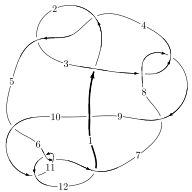
\includegraphics[width=112pt]{../../../GIT/diagram.site/Diagrams/png/899_12a_0098.png}\\
\ \ \ A knot diagram\footnotemark}&
\allowdisplaybreaks
\textbf{Linearized knot diagam} \\
\cline{2-2}
 &
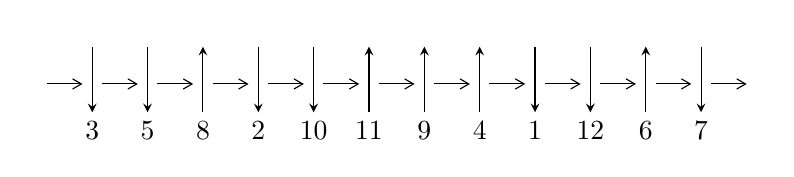
\begin{tikzpicture}[x=20pt, y=17pt]
	% nodes
	\node (C0) at (0, 0) {};
	\node (C1) at (1, 0) {};
	\node (C1U) at (1, +1) {};
	\node (C1D) at (1, -1) {3};

	\node (C2) at (2, 0) {};
	\node (C2U) at (2, +1) {};
	\node (C2D) at (2, -1) {5};

	\node (C3) at (3, 0) {};
	\node (C3U) at (3, +1) {};
	\node (C3D) at (3, -1) {8};

	\node (C4) at (4, 0) {};
	\node (C4U) at (4, +1) {};
	\node (C4D) at (4, -1) {2};

	\node (C5) at (5, 0) {};
	\node (C5U) at (5, +1) {};
	\node (C5D) at (5, -1) {10};

	\node (C6) at (6, 0) {};
	\node (C6U) at (6, +1) {};
	\node (C6D) at (6, -1) {11};

	\node (C7) at (7, 0) {};
	\node (C7U) at (7, +1) {};
	\node (C7D) at (7, -1) {9};

	\node (C8) at (8, 0) {};
	\node (C8U) at (8, +1) {};
	\node (C8D) at (8, -1) {4};

	\node (C9) at (9, 0) {};
	\node (C9U) at (9, +1) {};
	\node (C9D) at (9, -1) {1};

	\node (C10) at (10, 0) {};
	\node (C10U) at (10, +1) {};
	\node (C10D) at (10, -1) {12};

	\node (C11) at (11, 0) {};
	\node (C11U) at (11, +1) {};
	\node (C11D) at (11, -1) {6};

	\node (C12) at (12, 0) {};
	\node (C12U) at (12, +1) {};
	\node (C12D) at (12, -1) {7};
	\node (C13) at (13, 0) {};

	% arrows
	\draw[->,>={angle 60}]
	(C0) edge (C1) (C1) edge (C2) (C2) edge (C3) (C3) edge (C4) (C4) edge (C5) (C5) edge (C6) (C6) edge (C7) (C7) edge (C8) (C8) edge (C9) (C9) edge (C10) (C10) edge (C11) (C11) edge (C12) (C12) edge (C13) ;	\draw[->,>=stealth]
	(C1U) edge (C1D) (C2U) edge (C2D) (C3D) edge (C3U) (C4U) edge (C4D) (C5U) edge (C5D) (C6D) edge (C6U) (C7D) edge (C7U) (C8D) edge (C8U) (C9U) edge (C9D) (C10U) edge (C10D) (C11D) edge (C11U) (C12U) edge (C12D) ;
	\end{tikzpicture} \\
\hhline{~~} \\& 
\textbf{Solving Sequence} \\ \cline{2-2} 
 &
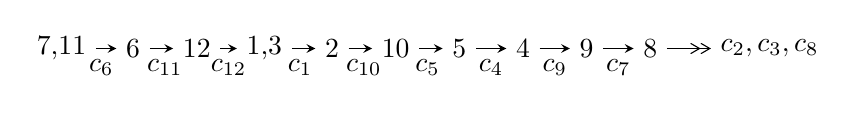
\begin{tikzpicture}[x=23pt, y=7pt]
	% node
	\node (A0) at (-1/8, 0) {7,11};
	\node (A1) at (1, 0) {6};
	\node (A2) at (2, 0) {12};
	\node (A3) at (49/16, 0) {1,3};
	\node (A4) at (33/8, 0) {2};
	\node (A5) at (41/8, 0) {10};
	\node (A6) at (49/8, 0) {5};
	\node (A7) at (57/8, 0) {4};
	\node (A8) at (65/8, 0) {9};
	\node (A9) at (73/8, 0) {8};
	\node (C1) at (1/2, -1) {$c_{6}$};
	\node (C2) at (3/2, -1) {$c_{11}$};
	\node (C3) at (5/2, -1) {$c_{12}$};
	\node (C4) at (29/8, -1) {$c_{1}$};
	\node (C5) at (37/8, -1) {$c_{10}$};
	\node (C6) at (45/8, -1) {$c_{5}$};
	\node (C7) at (53/8, -1) {$c_{4}$};
	\node (C8) at (61/8, -1) {$c_{9}$};
	\node (C9) at (69/8, -1) {$c_{7}$};
	\node (A10) at (11, 0) {$c_{2},c_{3},c_{8}$};

	% edge
	\draw[->,>=stealth]	
	(A0) edge (A1) (A1) edge (A2) (A2) edge (A3) (A3) edge (A4) (A4) edge (A5) (A5) edge (A6) (A6) edge (A7) (A7) edge (A8) (A8) edge (A9) ;
	\draw[->>,>={angle 60}]	
	(A9) edge (A10);
\end{tikzpicture} \\ 

\end{tabular} \\

\footnotetext{
The image of knot diagram is generated by the software ``\textbf{Draw programme}" developed by Andrew Bartholomew(\url{http://www.layer8.co.uk/maths/draw/index.htm\#Running-draw}), where we modified some parts for our purpose(\url{https://github.com/CATsTAILs/LinksPainter}).
}\phantom \\ \newline 
\centering \textbf{Ideals for irreducible components\footnotemark of $X_{\text{par}}$} 
 
\begin{align*}
I^u_{1}&=\langle 
u^{99}-2 u^{98}+\cdots+b+1,\;u^{98}- u^{97}+\cdots+a+1,\;u^{100}-2 u^{99}+\cdots+3 u-1\rangle \\
I^u_{2}&=\langle 
b,\;u^2+a- u+1,\;u^5- u^4+2 u^3- u^2+u-1\rangle \\
\\
\end{align*}
\raggedright * 2 irreducible components of $\dim_{\mathbb{C}}=0$, with total 105 representations.\\
\footnotetext{All coefficients of polynomials are rational numbers. But the coefficients are sometimes approximated in decimal forms when there is not enough margin.}
\newpage
\renewcommand{\arraystretch}{1}
\centering \section*{I. $I^u_{1}= \langle u^{99}-2 u^{98}+\cdots+b+1,\;u^{98}- u^{97}+\cdots+a+1,\;u^{100}-2 u^{99}+\cdots+3 u-1 \rangle$}
\flushleft \textbf{(i) Arc colorings}\\
\begin{tabular}{m{7pt} m{180pt} m{7pt} m{180pt} }
\flushright $a_{7}=$&$\begin{pmatrix}1\\0\end{pmatrix}$ \\
\flushright $a_{11}=$&$\begin{pmatrix}0\\u\end{pmatrix}$ \\
\flushright $a_{6}=$&$\begin{pmatrix}1\\u^2\end{pmatrix}$ \\
\flushright $a_{12}=$&$\begin{pmatrix}u\\u^3+u\end{pmatrix}$ \\
\flushright $a_{1}=$&$\begin{pmatrix}- u^3\\u^3+u\end{pmatrix}$ \\
\flushright $a_{3}=$&$\begin{pmatrix}- u^{98}+u^{97}+\cdots+2 u-1\\- u^{99}+2 u^{98}+\cdots+2 u-1\end{pmatrix}$ \\
\flushright $a_{2}=$&$\begin{pmatrix}- u^{95}+u^{94}+\cdots+4 u-2\\- u^{52}-14 u^{50}+\cdots-2 u^3+2 u^2\end{pmatrix}$ \\
\flushright $a_{10}=$&$\begin{pmatrix}u^3\\u^5+u^3+u\end{pmatrix}$ \\
\flushright $a_{5}=$&$\begin{pmatrix}- u^6- u^4+1\\- u^8-2 u^6-2 u^4\end{pmatrix}$ \\
\flushright $a_{4}=$&$\begin{pmatrix}u^{98}- u^{97}+\cdots+5 u-2\\u^{99}-2 u^{98}+\cdots-3 u+1\end{pmatrix}$ \\
\flushright $a_{9}=$&$\begin{pmatrix}u^{11}+2 u^9+2 u^7+u^3\\- u^{11}-3 u^9-4 u^7- u^5+u^3+u\end{pmatrix}$ \\
\flushright $a_{8}=$&$\begin{pmatrix}u^{22}+5 u^{20}+12 u^{18}+15 u^{16}+10 u^{14}+2 u^{12}- u^8- u^6- u^4+1\\- u^{22}-6 u^{20}-17 u^{18}-26 u^{16}-20 u^{14}+13 u^{10}+10 u^8+u^6-2 u^4- u^2\end{pmatrix}$\\&\end{tabular}
\flushleft \textbf{(ii) Obstruction class $= -1$}\\~\\
\flushleft \textbf{(iii) Cusp Shapes $= 4 u^{99}-15 u^{98}+\cdots-24 u+7$}\\~\\
\newpage\renewcommand{\arraystretch}{1}
\flushleft \textbf{(iv) u-Polynomials at the component}\newline \\
\begin{tabular}{m{50pt}|m{274pt}}
Crossings & \hspace{64pt}u-Polynomials at each crossing \\
\hline $$\begin{aligned}c_{1}\end{aligned}$$&$\begin{aligned}
&u^{100}+54 u^{99}+\cdots+5 u+1
\end{aligned}$\\
\hline $$\begin{aligned}c_{2},c_{4}\end{aligned}$$&$\begin{aligned}
&u^{100}-6 u^{99}+\cdots+5 u-1
\end{aligned}$\\
\hline $$\begin{aligned}c_{3},c_{8}\end{aligned}$$&$\begin{aligned}
&u^{100}+u^{99}+\cdots+64 u+32
\end{aligned}$\\
\hline $$\begin{aligned}c_{5},c_{12}\end{aligned}$$&$\begin{aligned}
&u^{100}+2 u^{99}+\cdots-9 u-1
\end{aligned}$\\
\hline $$\begin{aligned}c_{6},c_{11}\end{aligned}$$&$\begin{aligned}
&u^{100}-2 u^{99}+\cdots+3 u-1
\end{aligned}$\\
\hline $$\begin{aligned}c_{7}\end{aligned}$$&$\begin{aligned}
&u^{100}-33 u^{99}+\cdots-23040 u+1024
\end{aligned}$\\
\hline $$\begin{aligned}c_{9}\end{aligned}$$&$\begin{aligned}
&u^{100}-14 u^{99}+\cdots-5687 u+409
\end{aligned}$\\
\hline $$\begin{aligned}c_{10}\end{aligned}$$&$\begin{aligned}
&u^{100}+54 u^{99}+\cdots+5 u+1
\end{aligned}$\\
\hline
\end{tabular}\\~\\
\newpage\renewcommand{\arraystretch}{1}
\flushleft \textbf{(v) Riley Polynomials at the component}\newline \\
\begin{tabular}{m{50pt}|m{274pt}}
Crossings & \hspace{64pt}Riley Polynomials at each crossing \\
\hline $$\begin{aligned}c_{1}\end{aligned}$$&$\begin{aligned}
&y^{100}-10 y^{99}+\cdots+11 y+1
\end{aligned}$\\
\hline $$\begin{aligned}c_{2},c_{4}\end{aligned}$$&$\begin{aligned}
&y^{100}-54 y^{99}+\cdots-5 y+1
\end{aligned}$\\
\hline $$\begin{aligned}c_{3},c_{8}\end{aligned}$$&$\begin{aligned}
&y^{100}-33 y^{99}+\cdots-23040 y+1024
\end{aligned}$\\
\hline $$\begin{aligned}c_{5},c_{12}\end{aligned}$$&$\begin{aligned}
&y^{100}-82 y^{99}+\cdots+149 y+1
\end{aligned}$\\
\hline $$\begin{aligned}c_{6},c_{11}\end{aligned}$$&$\begin{aligned}
&y^{100}+54 y^{99}+\cdots+5 y+1
\end{aligned}$\\
\hline $$\begin{aligned}c_{7}\end{aligned}$$&$\begin{aligned}
&y^{100}+59 y^{99}+\cdots-17432576 y+1048576
\end{aligned}$\\
\hline $$\begin{aligned}c_{9}\end{aligned}$$&$\begin{aligned}
&y^{100}-22 y^{99}+\cdots+9736769 y+167281
\end{aligned}$\\
\hline $$\begin{aligned}c_{10}\end{aligned}$$&$\begin{aligned}
&y^{100}-14 y^{99}+\cdots-3 y+1
\end{aligned}$\\
\hline
\end{tabular}\\~\\
\newpage\flushleft \textbf{(vi) Complex Volumes and Cusp Shapes}
$$\begin{array}{c|c|c}  
\text{Solutions to }I^u_{1}& \I (\text{vol} + \sqrt{-1}CS) & \text{Cusp shape}\\
 \hline 
\begin{aligned}
u &= -0.487101 + 0.887376 I \\
a &= -0.64534 + 1.56978 I \\
b &= \phantom{-}0.237262 + 0.339303 I\end{aligned}
 & -2.85974 - 3.13345 I & \phantom{-0.000000 } 0 \\ \hline\begin{aligned}
u &= -0.487101 - 0.887376 I \\
a &= -0.64534 - 1.56978 I \\
b &= \phantom{-}0.237262 - 0.339303 I\end{aligned}
 & -2.85974 + 3.13345 I & \phantom{-0.000000 } 0 \\ \hline\begin{aligned}
u &= \phantom{-}0.512139 + 0.884085 I \\
a &= \phantom{-}0.85983 - 1.96917 I \\
b &= \phantom{-}2.12852 + 0.82152 I\end{aligned}
 & -2.46262 + 5.68656 I & \phantom{-0.000000 } 0 \\ \hline\begin{aligned}
u &= \phantom{-}0.512139 - 0.884085 I \\
a &= \phantom{-}0.85983 + 1.96917 I \\
b &= \phantom{-}2.12852 - 0.82152 I\end{aligned}
 & -2.46262 - 5.68656 I & \phantom{-0.000000 } 0 \\ \hline\begin{aligned}
u &= -0.535428 + 0.873146 I \\
a &= -0.102230 + 0.397660 I \\
b &= \phantom{-}0.983013 + 0.192627 I\end{aligned}
 & \phantom{-}1.71894 - 6.57445 I & \phantom{-0.000000 } 0 \\ \hline\begin{aligned}
u &= -0.535428 - 0.873146 I \\
a &= -0.102230 - 0.397660 I \\
b &= \phantom{-}0.983013 - 0.192627 I\end{aligned}
 & \phantom{-}1.71894 + 6.57445 I & \phantom{-0.000000 } 0 \\ \hline\begin{aligned}
u &= \phantom{-}0.061097 + 1.022580 I \\
a &= -0.064633 + 0.226670 I \\
b &= \phantom{-}0.076689 + 0.466636 I\end{aligned}
 & -2.29873 + 2.42299 I & \phantom{-0.000000 } 0 \\ \hline\begin{aligned}
u &= \phantom{-}0.061097 - 1.022580 I \\
a &= -0.064633 - 0.226670 I \\
b &= \phantom{-}0.076689 - 0.466636 I\end{aligned}
 & -2.29873 - 2.42299 I & \phantom{-0.000000 } 0 \\ \hline\begin{aligned}
u &= -0.014877 + 1.027310 I \\
a &= -1.90233 + 0.83604 I \\
b &= \phantom{-}0.90903 - 1.15393 I\end{aligned}
 & -6.01004 - 1.32650 I & \phantom{-0.000000 } 0 \\ \hline\begin{aligned}
u &= -0.014877 - 1.027310 I \\
a &= -1.90233 - 0.83604 I \\
b &= \phantom{-}0.90903 + 1.15393 I\end{aligned}
 & -6.01004 + 1.32650 I & \phantom{-0.000000 } 0\\
 \hline 
 \end{array}$$\newpage$$\begin{array}{c|c|c}  
\text{Solutions to }I^u_{1}& \I (\text{vol} + \sqrt{-1}CS) & \text{Cusp shape}\\
 \hline 
\begin{aligned}
u &= \phantom{-}0.281502 + 0.988175 I \\
a &= \phantom{-}1.171170 + 0.536052 I \\
b &= -0.644688 - 0.009719 I\end{aligned}
 & -0.57782 + 2.38994 I & \phantom{-0.000000 } 0 \\ \hline\begin{aligned}
u &= \phantom{-}0.281502 - 0.988175 I \\
a &= \phantom{-}1.171170 - 0.536052 I \\
b &= -0.644688 + 0.009719 I\end{aligned}
 & -0.57782 - 2.38994 I & \phantom{-0.000000 } 0 \\ \hline\begin{aligned}
u &= -0.544624 + 0.786486 I \\
a &= -0.96241 - 1.40714 I \\
b &= -1.38076 + 0.76706 I\end{aligned}
 & \phantom{-}4.62351 - 4.68716 I & \phantom{-0.000000 } 0 \\ \hline\begin{aligned}
u &= -0.544624 - 0.786486 I \\
a &= -0.96241 + 1.40714 I \\
b &= -1.38076 - 0.76706 I\end{aligned}
 & \phantom{-}4.62351 + 4.68716 I & \phantom{-0.000000 } 0 \\ \hline\begin{aligned}
u &= -0.549344 + 0.893780 I \\
a &= -0.75864 - 1.80248 I \\
b &= -2.01660 + 0.64147 I\end{aligned}
 & -0.99980 - 11.63300 I & \phantom{-0.000000 } 0 \\ \hline\begin{aligned}
u &= -0.549344 - 0.893780 I \\
a &= -0.75864 + 1.80248 I \\
b &= -2.01660 - 0.64147 I\end{aligned}
 & -0.99980 + 11.63300 I & \phantom{-0.000000 } 0 \\ \hline\begin{aligned}
u &= \phantom{-}0.440563 + 0.839915 I \\
a &= \phantom{-}0.601924 + 0.493045 I \\
b &= -0.771261 + 0.570745 I\end{aligned}
 & -0.05742 + 1.93114 I & \phantom{-0.000000 } 0 \\ \hline\begin{aligned}
u &= \phantom{-}0.440563 - 0.839915 I \\
a &= \phantom{-}0.601924 - 0.493045 I \\
b &= -0.771261 - 0.570745 I\end{aligned}
 & -0.05742 - 1.93114 I & \phantom{-0.000000 } 0 \\ \hline\begin{aligned}
u &= \phantom{-}0.055568 + 1.074490 I \\
a &= \phantom{-}1.82687 + 0.75760 I \\
b &= -1.10849 - 0.96099 I\end{aligned}
 & -5.21910 + 6.98392 I & \phantom{-0.000000 } 0 \\ \hline\begin{aligned}
u &= \phantom{-}0.055568 - 1.074490 I \\
a &= \phantom{-}1.82687 - 0.75760 I \\
b &= -1.10849 + 0.96099 I\end{aligned}
 & -5.21910 - 6.98392 I & \phantom{-0.000000 } 0\\
 \hline 
 \end{array}$$\newpage$$\begin{array}{c|c|c}  
\text{Solutions to }I^u_{1}& \I (\text{vol} + \sqrt{-1}CS) & \text{Cusp shape}\\
 \hline 
\begin{aligned}
u &= -0.544396 + 0.739925 I \\
a &= \phantom{-}0.072681 + 1.149840 I \\
b &= \phantom{-}1.49172 + 0.43095 I\end{aligned}
 & \phantom{-}4.75608 + 0.29953 I & \phantom{-0.000000 } 0 \\ \hline\begin{aligned}
u &= -0.544396 - 0.739925 I \\
a &= \phantom{-}0.072681 - 1.149840 I \\
b &= \phantom{-}1.49172 - 0.43095 I\end{aligned}
 & \phantom{-}4.75608 - 0.29953 I & \phantom{-0.000000 } 0 \\ \hline\begin{aligned}
u &= \phantom{-}0.481773 + 0.978864 I \\
a &= \phantom{-}0.50337 + 1.72394 I \\
b &= -0.521962 + 0.138752 I\end{aligned}
 & -2.30351 - 1.49233 I & \phantom{-0.000000 } 0 \\ \hline\begin{aligned}
u &= \phantom{-}0.481773 - 0.978864 I \\
a &= \phantom{-}0.50337 - 1.72394 I \\
b &= -0.521962 - 0.138752 I\end{aligned}
 & -2.30351 + 1.49233 I & \phantom{-0.000000 } 0 \\ \hline\begin{aligned}
u &= \phantom{-}0.435072 + 0.741485 I \\
a &= \phantom{-}1.233090 - 0.445011 I \\
b &= \phantom{-}0.325832 + 1.179420 I\end{aligned}
 & \phantom{-}0.21908 + 1.78940 I & \phantom{-}0.70752 - 5.47893 I \\ \hline\begin{aligned}
u &= \phantom{-}0.435072 - 0.741485 I \\
a &= \phantom{-}1.233090 + 0.445011 I \\
b &= \phantom{-}0.325832 - 1.179420 I\end{aligned}
 & \phantom{-}0.21908 - 1.78940 I & \phantom{-}0.70752 + 5.47893 I \\ \hline\begin{aligned}
u &= \phantom{-}0.824459 + 0.135370 I \\
a &= -0.035450 - 1.023230 I \\
b &= -2.22486 + 1.32612 I\end{aligned}
 & -4.76000 - 12.04300 I & -3.90865 + 7.83863 I \\ \hline\begin{aligned}
u &= \phantom{-}0.824459 - 0.135370 I \\
a &= -0.035450 + 1.023230 I \\
b &= -2.22486 - 1.32612 I\end{aligned}
 & -4.76000 + 12.04300 I & -3.90865 - 7.83863 I \\ \hline\begin{aligned}
u &= -0.825648 + 0.079549 I \\
a &= \phantom{-}0.654212 + 0.474789 I \\
b &= -0.026542 + 0.835432 I\end{aligned}
 & -6.39732 - 2.29666 I & -5.74508 + 3.83085 I \\ \hline\begin{aligned}
u &= -0.825648 - 0.079549 I \\
a &= \phantom{-}0.654212 - 0.474789 I \\
b &= -0.026542 - 0.835432 I\end{aligned}
 & -6.39732 + 2.29666 I & -5.74508 - 3.83085 I\\
 \hline 
 \end{array}$$\newpage$$\begin{array}{c|c|c}  
\text{Solutions to }I^u_{1}& \I (\text{vol} + \sqrt{-1}CS) & \text{Cusp shape}\\
 \hline 
\begin{aligned}
u &= -0.578115 + 0.594628 I \\
a &= \phantom{-}0.66753 + 1.49885 I \\
b &= \phantom{-}1.70331 + 0.41644 I\end{aligned}
 & -0.16037 + 7.14748 I & -0.19098 - 4.78426 I \\ \hline\begin{aligned}
u &= -0.578115 - 0.594628 I \\
a &= \phantom{-}0.66753 - 1.49885 I \\
b &= \phantom{-}1.70331 - 0.41644 I\end{aligned}
 & -0.16037 - 7.14748 I & -0.19098 + 4.78426 I \\ \hline\begin{aligned}
u &= -0.543322 + 0.623428 I \\
a &= -0.500926 - 0.937819 I \\
b &= -0.592010 + 0.346478 I\end{aligned}
 & \phantom{-}2.41952 + 2.21533 I & \phantom{-}3.55808 - 1.03686 I \\ \hline\begin{aligned}
u &= -0.543322 - 0.623428 I \\
a &= -0.500926 + 0.937819 I \\
b &= -0.592010 - 0.346478 I\end{aligned}
 & \phantom{-}2.41952 - 2.21533 I & \phantom{-}3.55808 + 1.03686 I \\ \hline\begin{aligned}
u &= \phantom{-}0.808693 + 0.134012 I \\
a &= -0.042565 + 0.155136 I \\
b &= \phantom{-}1.43091 - 0.46157 I\end{aligned}
 & -1.75864 - 6.90513 I & -0.71442 + 4.85382 I \\ \hline\begin{aligned}
u &= \phantom{-}0.808693 - 0.134012 I \\
a &= -0.042565 - 0.155136 I \\
b &= \phantom{-}1.43091 + 0.46157 I\end{aligned}
 & -1.75864 + 6.90513 I & -0.71442 - 4.85382 I \\ \hline\begin{aligned}
u &= -0.808227 + 0.119737 I \\
a &= \phantom{-}0.001013 - 1.118540 I \\
b &= \phantom{-}2.18276 + 1.75899 I\end{aligned}
 & -5.96708 + 5.74079 I & -5.45196 - 4.06598 I \\ \hline\begin{aligned}
u &= -0.808227 - 0.119737 I \\
a &= \phantom{-}0.001013 + 1.118540 I \\
b &= \phantom{-}2.18276 - 1.75899 I\end{aligned}
 & -5.96708 - 5.74079 I & -5.45196 + 4.06598 I \\ \hline\begin{aligned}
u &= \phantom{-}0.432154 + 1.101560 I \\
a &= \phantom{-}1.41814 - 0.54319 I \\
b &= -0.682213 + 0.652652 I\end{aligned}
 & -0.54978 + 2.70789 I & \phantom{-0.000000 } 0 \\ \hline\begin{aligned}
u &= \phantom{-}0.432154 - 1.101560 I \\
a &= \phantom{-}1.41814 + 0.54319 I \\
b &= -0.682213 - 0.652652 I\end{aligned}
 & -0.54978 - 2.70789 I & \phantom{-0.000000 } 0\\
 \hline 
 \end{array}$$\newpage$$\begin{array}{c|c|c}  
\text{Solutions to }I^u_{1}& \I (\text{vol} + \sqrt{-1}CS) & \text{Cusp shape}\\
 \hline 
\begin{aligned}
u &= \phantom{-}0.804661 + 0.108864 I \\
a &= -0.773190 + 0.547526 I \\
b &= -0.216473 + 0.828174 I\end{aligned}
 & -6.30355 - 2.94906 I & -5.62609 + 3.05585 I \\ \hline\begin{aligned}
u &= \phantom{-}0.804661 - 0.108864 I \\
a &= -0.773190 - 0.547526 I \\
b &= -0.216473 - 0.828174 I\end{aligned}
 & -6.30355 + 2.94906 I & -5.62609 - 3.05585 I \\ \hline\begin{aligned}
u &= -0.800011\phantom{ +0.000000I} \\
a &= \phantom{-}0.579040\phantom{ +0.000000I} \\
b &= -0.453790\phantom{ +0.000000I}\end{aligned}
 & -3.31846\phantom{ +0.000000I} & \phantom{-}3.13170\phantom{ +0.000000I} \\ \hline\begin{aligned}
u &= \phantom{-}0.362513 + 1.145170 I \\
a &= -1.23658 + 1.82457 I \\
b &= \phantom{-}0.406691 - 0.980808 I\end{aligned}
 & -1.70065 - 1.90512 I & \phantom{-0.000000 } 0 \\ \hline\begin{aligned}
u &= \phantom{-}0.362513 - 1.145170 I \\
a &= -1.23658 - 1.82457 I \\
b &= \phantom{-}0.406691 + 0.980808 I\end{aligned}
 & -1.70065 + 1.90512 I & \phantom{-0.000000 } 0 \\ \hline\begin{aligned}
u &= -0.789568 + 0.093306 I \\
a &= \phantom{-}0.195595 + 0.130891 I \\
b &= -1.317430 - 0.428608 I\end{aligned}
 & -3.06121 + 1.43669 I & -2.47302 - 0.11715 I \\ \hline\begin{aligned}
u &= -0.789568 - 0.093306 I \\
a &= \phantom{-}0.195595 - 0.130891 I \\
b &= -1.317430 + 0.428608 I\end{aligned}
 & -3.06121 - 1.43669 I & -2.47302 + 0.11715 I \\ \hline\begin{aligned}
u &= \phantom{-}0.498648 + 0.587209 I \\
a &= -0.62990 + 1.82971 I \\
b &= -1.73628 + 0.37315 I\end{aligned}
 & -1.64770 - 1.50599 I & -1.92217 + 0.80453 I \\ \hline\begin{aligned}
u &= \phantom{-}0.498648 - 0.587209 I \\
a &= -0.62990 - 1.82971 I \\
b &= -1.73628 - 0.37315 I\end{aligned}
 & -1.64770 + 1.50599 I & -1.92217 - 0.80453 I \\ \hline\begin{aligned}
u &= -0.435541 + 1.155600 I \\
a &= \phantom{-}0.09357 + 3.60800 I \\
b &= \phantom{-}1.11804 - 1.66899 I\end{aligned}
 & -4.86062 - 2.24576 I & \phantom{-0.000000 } 0\\
 \hline 
 \end{array}$$\newpage$$\begin{array}{c|c|c}  
\text{Solutions to }I^u_{1}& \I (\text{vol} + \sqrt{-1}CS) & \text{Cusp shape}\\
 \hline 
\begin{aligned}
u &= -0.435541 - 1.155600 I \\
a &= \phantom{-}0.09357 - 3.60800 I \\
b &= \phantom{-}1.11804 + 1.66899 I\end{aligned}
 & -4.86062 + 2.24576 I & \phantom{-0.000000 } 0 \\ \hline\begin{aligned}
u &= \phantom{-}0.737955 + 0.179606 I \\
a &= -0.253244 - 1.053450 I \\
b &= -0.82591 + 1.17880 I\end{aligned}
 & \phantom{-}2.13680 - 5.42672 I & \phantom{-}1.72948 + 6.28208 I \\ \hline\begin{aligned}
u &= \phantom{-}0.737955 - 0.179606 I \\
a &= -0.253244 + 1.053450 I \\
b &= -0.82591 - 1.17880 I\end{aligned}
 & \phantom{-}2.13680 + 5.42672 I & \phantom{-}1.72948 - 6.28208 I \\ \hline\begin{aligned}
u &= \phantom{-}0.495377 + 1.145420 I \\
a &= \phantom{-}0.81566 + 2.36176 I \\
b &= -1.45498 - 0.50738 I\end{aligned}
 & \phantom{-}0.07482 + 5.02620 I & \phantom{-0.000000 } 0 \\ \hline\begin{aligned}
u &= \phantom{-}0.495377 - 1.145420 I \\
a &= \phantom{-}0.81566 - 2.36176 I \\
b &= -1.45498 + 0.50738 I\end{aligned}
 & \phantom{-}0.07482 - 5.02620 I & \phantom{-0.000000 } 0 \\ \hline\begin{aligned}
u &= \phantom{-}0.453852 + 1.167430 I \\
a &= \phantom{-}0.375656 - 0.273528 I \\
b &= \phantom{-}0.587582 - 0.060312 I\end{aligned}
 & -6.15358 + 4.16473 I & \phantom{-0.000000 } 0 \\ \hline\begin{aligned}
u &= \phantom{-}0.453852 - 1.167430 I \\
a &= \phantom{-}0.375656 + 0.273528 I \\
b &= \phantom{-}0.587582 + 0.060312 I\end{aligned}
 & -6.15358 - 4.16473 I & \phantom{-0.000000 } 0 \\ \hline\begin{aligned}
u &= -0.472406 + 1.164010 I \\
a &= -2.77759 - 2.12300 I \\
b &= \phantom{-}0.55876 + 2.02590 I\end{aligned}
 & -4.58329 - 5.97967 I & \phantom{-0.000000 } 0 \\ \hline\begin{aligned}
u &= -0.472406 - 1.164010 I \\
a &= -2.77759 + 2.12300 I \\
b &= \phantom{-}0.55876 - 2.02590 I\end{aligned}
 & -4.58329 + 5.97967 I & \phantom{-0.000000 } 0 \\ \hline\begin{aligned}
u &= \phantom{-}0.507155 + 1.162800 I \\
a &= \phantom{-}0.91044 - 2.82854 I \\
b &= \phantom{-}0.76397 + 1.44828 I\end{aligned}
 & -0.72084 + 10.09420 I & \phantom{-0.000000 } 0\\
 \hline 
 \end{array}$$\newpage$$\begin{array}{c|c|c}  
\text{Solutions to }I^u_{1}& \I (\text{vol} + \sqrt{-1}CS) & \text{Cusp shape}\\
 \hline 
\begin{aligned}
u &= \phantom{-}0.507155 - 1.162800 I \\
a &= \phantom{-}0.91044 + 2.82854 I \\
b &= \phantom{-}0.76397 - 1.44828 I\end{aligned}
 & -0.72084 - 10.09420 I & \phantom{-0.000000 } 0 \\ \hline\begin{aligned}
u &= \phantom{-}0.381540 + 1.214470 I \\
a &= \phantom{-}1.90375 + 0.08418 I \\
b &= -1.32632 + 0.72565 I\end{aligned}
 & -5.81050 - 2.87951 I & \phantom{-0.000000 } 0 \\ \hline\begin{aligned}
u &= \phantom{-}0.381540 - 1.214470 I \\
a &= \phantom{-}1.90375 - 0.08418 I \\
b &= -1.32632 - 0.72565 I\end{aligned}
 & -5.81050 + 2.87951 I & \phantom{-0.000000 } 0 \\ \hline\begin{aligned}
u &= -0.407140 + 1.208730 I \\
a &= -1.92802 + 0.11186 I \\
b &= \phantom{-}1.24526 + 0.74300 I\end{aligned}
 & -6.90359 - 2.70005 I & \phantom{-0.000000 } 0 \\ \hline\begin{aligned}
u &= -0.407140 - 1.208730 I \\
a &= -1.92802 - 0.11186 I \\
b &= \phantom{-}1.24526 - 0.74300 I\end{aligned}
 & -6.90359 + 2.70005 I & \phantom{-0.000000 } 0 \\ \hline\begin{aligned}
u &= \phantom{-}0.584288 + 0.428222 I \\
a &= \phantom{-}0.331398 + 1.168580 I \\
b &= \phantom{-}1.042000 + 0.223440 I\end{aligned}
 & -0.74199 + 5.73096 I & -0.46933 - 5.70886 I \\ \hline\begin{aligned}
u &= \phantom{-}0.584288 - 0.428222 I \\
a &= \phantom{-}0.331398 - 1.168580 I \\
b &= \phantom{-}1.042000 - 0.223440 I\end{aligned}
 & -0.74199 - 5.73096 I & -0.46933 + 5.70886 I \\ \hline\begin{aligned}
u &= -0.390582 + 1.215960 I \\
a &= \phantom{-}3.52756 + 1.57398 I \\
b &= -1.95856 - 1.94901 I\end{aligned}
 & -9.96791 + 1.65394 I & \phantom{-0.000000 } 0 \\ \hline\begin{aligned}
u &= -0.390582 - 1.215960 I \\
a &= \phantom{-}3.52756 - 1.57398 I \\
b &= -1.95856 + 1.94901 I\end{aligned}
 & -9.96791 - 1.65394 I & \phantom{-0.000000 } 0 \\ \hline\begin{aligned}
u &= \phantom{-}0.397348 + 1.215000 I \\
a &= -0.153885 + 0.492319 I \\
b &= \phantom{-}0.220508 - 1.046930 I\end{aligned}
 & -10.25340 + 1.17144 I & \phantom{-0.000000 } 0\\
 \hline 
 \end{array}$$\newpage$$\begin{array}{c|c|c}  
\text{Solutions to }I^u_{1}& \I (\text{vol} + \sqrt{-1}CS) & \text{Cusp shape}\\
 \hline 
\begin{aligned}
u &= \phantom{-}0.397348 - 1.215000 I \\
a &= -0.153885 - 0.492319 I \\
b &= \phantom{-}0.220508 + 1.046930 I\end{aligned}
 & -10.25340 - 1.17144 I & \phantom{-0.000000 } 0 \\ \hline\begin{aligned}
u &= \phantom{-}0.378815 + 1.225050 I \\
a &= -3.23541 + 1.04754 I \\
b &= \phantom{-}2.06321 - 1.49338 I\end{aligned}
 & -8.88797 - 7.96569 I & \phantom{-0.000000 } 0 \\ \hline\begin{aligned}
u &= \phantom{-}0.378815 - 1.225050 I \\
a &= -3.23541 - 1.04754 I \\
b &= \phantom{-}2.06321 + 1.49338 I\end{aligned}
 & -8.88797 + 7.96569 I & \phantom{-0.000000 } 0 \\ \hline\begin{aligned}
u &= \phantom{-}0.680366 + 0.201848 I \\
a &= -0.077511 + 0.618875 I \\
b &= \phantom{-}1.313020 - 0.208942 I\end{aligned}
 & \phantom{-}2.79666 - 0.53221 I & \phantom{-}3.73788 - 0.05845 I \\ \hline\begin{aligned}
u &= \phantom{-}0.680366 - 0.201848 I \\
a &= -0.077511 - 0.618875 I \\
b &= \phantom{-}1.313020 + 0.208942 I\end{aligned}
 & \phantom{-}2.79666 + 0.53221 I & \phantom{-}3.73788 + 0.05845 I \\ \hline\begin{aligned}
u &= -0.493166 + 1.196550 I \\
a &= -1.11383 + 1.86850 I \\
b &= \phantom{-}1.57907 - 0.45097 I\end{aligned}
 & -6.29130 - 6.13018 I & \phantom{-0.000000 } 0 \\ \hline\begin{aligned}
u &= -0.493166 - 1.196550 I \\
a &= -1.11383 - 1.86850 I \\
b &= \phantom{-}1.57907 + 0.45097 I\end{aligned}
 & -6.29130 + 6.13018 I & \phantom{-0.000000 } 0 \\ \hline\begin{aligned}
u &= -0.413146 + 1.227640 I \\
a &= -0.014578 + 0.657209 I \\
b &= \phantom{-}0.053942 - 1.014040 I\end{aligned}
 & -10.32580 - 6.60037 I & \phantom{-0.000000 } 0 \\ \hline\begin{aligned}
u &= -0.413146 - 1.227640 I \\
a &= -0.014578 - 0.657209 I \\
b &= \phantom{-}0.053942 + 1.014040 I\end{aligned}
 & -10.32580 + 6.60037 I & \phantom{-0.000000 } 0 \\ \hline\begin{aligned}
u &= -0.455587 + 1.212890 I \\
a &= -0.917999 + 0.410244 I \\
b &= \phantom{-}0.444463 - 0.011374 I\end{aligned}
 & -6.88676 - 4.49128 I & \phantom{-0.000000 } 0\\
 \hline 
 \end{array}$$\newpage$$\begin{array}{c|c|c}  
\text{Solutions to }I^u_{1}& \I (\text{vol} + \sqrt{-1}CS) & \text{Cusp shape}\\
 \hline 
\begin{aligned}
u &= -0.455587 - 1.212890 I \\
a &= -0.917999 - 0.410244 I \\
b &= \phantom{-}0.444463 + 0.011374 I\end{aligned}
 & -6.88676 + 4.49128 I & \phantom{-0.000000 } 0 \\ \hline\begin{aligned}
u &= \phantom{-}0.501005 + 1.199870 I \\
a &= \phantom{-}1.012660 - 0.468509 I \\
b &= \phantom{-}0.376071 + 0.795331 I\end{aligned}
 & -9.51720 + 7.72554 I & \phantom{-0.000000 } 0 \\ \hline\begin{aligned}
u &= \phantom{-}0.501005 - 1.199870 I \\
a &= \phantom{-}1.012660 + 0.468509 I \\
b &= \phantom{-}0.376071 - 0.795331 I\end{aligned}
 & -9.51720 - 7.72554 I & \phantom{-0.000000 } 0 \\ \hline\begin{aligned}
u &= \phantom{-}0.511051 + 1.196640 I \\
a &= \phantom{-}0.92636 + 1.94812 I \\
b &= -1.63284 - 0.49708 I\end{aligned}
 & -4.89488 + 11.74760 I & \phantom{-0.000000 } 0 \\ \hline\begin{aligned}
u &= \phantom{-}0.511051 - 1.196640 I \\
a &= \phantom{-}0.92636 - 1.94812 I \\
b &= -1.63284 + 0.49708 I\end{aligned}
 & -4.89488 - 11.74760 I & \phantom{-0.000000 } 0 \\ \hline\begin{aligned}
u &= -0.505714 + 1.199280 I \\
a &= \phantom{-}0.27473 - 4.54256 I \\
b &= -2.35444 + 1.89934 I\end{aligned}
 & -9.15153 - 10.55260 I & \phantom{-0.000000 } 0 \\ \hline\begin{aligned}
u &= -0.505714 - 1.199280 I \\
a &= \phantom{-}0.27473 + 4.54256 I \\
b &= -2.35444 - 1.89934 I\end{aligned}
 & -9.15153 + 10.55260 I & \phantom{-0.000000 } 0 \\ \hline\begin{aligned}
u &= \phantom{-}0.514998 + 1.202160 I \\
a &= -0.63872 - 4.05356 I \\
b &= \phantom{-}2.37010 + 1.41332 I\end{aligned}
 & -7.9226 + 16.9439 I & \phantom{-0.000000 } 0 \\ \hline\begin{aligned}
u &= \phantom{-}0.514998 - 1.202160 I \\
a &= -0.63872 + 4.05356 I \\
b &= \phantom{-}2.37010 - 1.41332 I\end{aligned}
 & -7.9226 - 16.9439 I & \phantom{-0.000000 } 0 \\ \hline\begin{aligned}
u &= -0.492233 + 1.213360 I \\
a &= -1.127970 - 0.340973 I \\
b &= -0.116806 + 0.827372 I\end{aligned}
 & -9.76185 - 2.48344 I & \phantom{-0.000000 } 0\\
 \hline 
 \end{array}$$\newpage$$\begin{array}{c|c|c}  
\text{Solutions to }I^u_{1}& \I (\text{vol} + \sqrt{-1}CS) & \text{Cusp shape}\\
 \hline 
\begin{aligned}
u &= -0.492233 - 1.213360 I \\
a &= -1.127970 + 0.340973 I \\
b &= -0.116806 - 0.827372 I\end{aligned}
 & -9.76185 + 2.48344 I & \phantom{-0.000000 } 0 \\ \hline\begin{aligned}
u &= -0.669706 + 0.085937 I \\
a &= \phantom{-}0.594226 - 0.989167 I \\
b &= -0.54335 + 1.59916 I\end{aligned}
 & -1.54837 + 1.65311 I & -2.30876 - 3.97340 I \\ \hline\begin{aligned}
u &= -0.669706 - 0.085937 I \\
a &= \phantom{-}0.594226 + 0.989167 I \\
b &= -0.54335 - 1.59916 I\end{aligned}
 & -1.54837 - 1.65311 I & -2.30876 + 3.97340 I \\ \hline\begin{aligned}
u &= \phantom{-}0.674398\phantom{ +0.000000I} \\
a &= -1.27425\phantom{ +0.000000I} \\
b &= -0.524099\phantom{ +0.000000I}\end{aligned}
 & -2.93668\phantom{ +0.000000I} & \phantom{-}0.594550\phantom{ +0.000000I} \\ \hline\begin{aligned}
u &= -0.397234 + 0.514555 I \\
a &= -0.43988 + 1.63914 I \\
b &= -0.698089 + 0.059413 I\end{aligned}
 & -1.95778 - 0.78971 I & -2.64817 - 0.48190 I \\ \hline\begin{aligned}
u &= -0.397234 - 0.514555 I \\
a &= -0.43988 - 1.63914 I \\
b &= -0.698089 - 0.059413 I\end{aligned}
 & -1.95778 + 0.78971 I & -2.64817 + 0.48190 I \\ \hline\begin{aligned}
u &= -0.263931 + 0.581955 I \\
a &= -0.72627 + 1.86741 I \\
b &= -0.564883 - 0.162134 I\end{aligned}
 & -1.93880 - 0.78358 I & -3.76235 - 2.11912 I \\ \hline\begin{aligned}
u &= -0.263931 - 0.581955 I \\
a &= -0.72627 - 1.86741 I \\
b &= -0.564883 + 0.162134 I\end{aligned}
 & -1.93880 + 0.78358 I & -3.76235 + 2.11912 I \\ \hline\begin{aligned}
u &= \phantom{-}0.537250 + 0.344396 I \\
a &= -0.064717 - 0.765608 I \\
b &= \phantom{-}0.092979 + 0.350954 I\end{aligned}
 & \phantom{-}1.59701 + 1.17190 I & \phantom{-}3.67208 - 1.41836 I \\ \hline\begin{aligned}
u &= \phantom{-}0.537250 - 0.344396 I \\
a &= -0.064717 + 0.765608 I \\
b &= \phantom{-}0.092979 - 0.350954 I\end{aligned}
 & \phantom{-}1.59701 - 1.17190 I & \phantom{-}3.67208 + 1.41836 I\\
 \hline 
 \end{array}$$\newpage\newpage\renewcommand{\arraystretch}{1}
\centering \section*{II. $I^u_{2}= \langle b,\;u^2+a- u+1,\;u^5- u^4+2 u^3- u^2+u-1 \rangle$}
\flushleft \textbf{(i) Arc colorings}\\
\begin{tabular}{m{7pt} m{180pt} m{7pt} m{180pt} }
\flushright $a_{7}=$&$\begin{pmatrix}1\\0\end{pmatrix}$ \\
\flushright $a_{11}=$&$\begin{pmatrix}0\\u\end{pmatrix}$ \\
\flushright $a_{6}=$&$\begin{pmatrix}1\\u^2\end{pmatrix}$ \\
\flushright $a_{12}=$&$\begin{pmatrix}u\\u^3+u\end{pmatrix}$ \\
\flushright $a_{1}=$&$\begin{pmatrix}- u^3\\u^3+u\end{pmatrix}$ \\
\flushright $a_{3}=$&$\begin{pmatrix}- u^2+u-1\\0\end{pmatrix}$ \\
\flushright $a_{2}=$&$\begin{pmatrix}- u^3- u^2+u-1\\u^3+u\end{pmatrix}$ \\
\flushright $a_{10}=$&$\begin{pmatrix}u^3\\u^4- u^3+u^2+1\end{pmatrix}$ \\
\flushright $a_{5}=$&$\begin{pmatrix}u^3\\- u^3- u\end{pmatrix}$ \\
\flushright $a_{4}=$&$\begin{pmatrix}- u^2+u-1\\0\end{pmatrix}$ \\
\flushright $a_{9}=$&$\begin{pmatrix}1\\0\end{pmatrix}$ \\
\flushright $a_{8}=$&$\begin{pmatrix}1\\0\end{pmatrix}$\\&\end{tabular}
\flushleft \textbf{(ii) Obstruction class $= 1$}\\~\\
\flushleft \textbf{(iii) Cusp Shapes $= -2 u^4+7 u^3-8 u^2+6 u-12$}\\~\\
\newpage\renewcommand{\arraystretch}{1}
\flushleft \textbf{(iv) u-Polynomials at the component}\newline \\
\begin{tabular}{m{50pt}|m{274pt}}
Crossings & \hspace{64pt}u-Polynomials at each crossing \\
\hline $$\begin{aligned}c_{1},c_{2}\end{aligned}$$&$\begin{aligned}
&(u-1)^5
\end{aligned}$\\
\hline $$\begin{aligned}c_{3},c_{7},c_{8}\end{aligned}$$&$\begin{aligned}
&u^5
\end{aligned}$\\
\hline $$\begin{aligned}c_{4}\end{aligned}$$&$\begin{aligned}
&(u+1)^5
\end{aligned}$\\
\hline $$\begin{aligned}c_{5},c_{9}\end{aligned}$$&$\begin{aligned}
&u^5+u^4-2 u^3- u^2+u-1
\end{aligned}$\\
\hline $$\begin{aligned}c_{6}\end{aligned}$$&$\begin{aligned}
&u^5- u^4+2 u^3- u^2+u-1
\end{aligned}$\\
\hline $$\begin{aligned}c_{10}\end{aligned}$$&$\begin{aligned}
&u^5-3 u^4+4 u^3- u^2- u+1
\end{aligned}$\\
\hline $$\begin{aligned}c_{11}\end{aligned}$$&$\begin{aligned}
&u^5+u^4+2 u^3+u^2+u+1
\end{aligned}$\\
\hline $$\begin{aligned}c_{12}\end{aligned}$$&$\begin{aligned}
&u^5- u^4-2 u^3+u^2+u+1
\end{aligned}$\\
\hline
\end{tabular}\\~\\
\newpage\renewcommand{\arraystretch}{1}
\flushleft \textbf{(v) Riley Polynomials at the component}\newline \\
\begin{tabular}{m{50pt}|m{274pt}}
Crossings & \hspace{64pt}Riley Polynomials at each crossing \\
\hline $$\begin{aligned}c_{1},c_{2},c_{4}\end{aligned}$$&$\begin{aligned}
&(y-1)^5
\end{aligned}$\\
\hline $$\begin{aligned}c_{3},c_{7},c_{8}\end{aligned}$$&$\begin{aligned}
&y^5
\end{aligned}$\\
\hline $$\begin{aligned}c_{5},c_{9},c_{12}\end{aligned}$$&$\begin{aligned}
&y^5-5 y^4+8 y^3-3 y^2- y-1
\end{aligned}$\\
\hline $$\begin{aligned}c_{6},c_{11}\end{aligned}$$&$\begin{aligned}
&y^5+3 y^4+4 y^3+y^2- y-1
\end{aligned}$\\
\hline $$\begin{aligned}c_{10}\end{aligned}$$&$\begin{aligned}
&y^5- y^4+8 y^3-3 y^2+3 y-1
\end{aligned}$\\
\hline
\end{tabular}\\~\\
\newpage\flushleft \textbf{(vi) Complex Volumes and Cusp Shapes}
$$\begin{array}{c|c|c}  
\text{Solutions to }I^u_{2}& \I (\text{vol} + \sqrt{-1}CS) & \text{Cusp shape}\\
 \hline 
\begin{aligned}
u &= -0.339110 + 0.822375 I \\
a &= -0.77780 + 1.38013 I \\
b &= \phantom{-0.000000 } 0\end{aligned}
 & -1.97403 - 1.53058 I & -5.00899 + 6.23673 I \\ \hline\begin{aligned}
u &= -0.339110 - 0.822375 I \\
a &= -0.77780 - 1.38013 I \\
b &= \phantom{-0.000000 } 0\end{aligned}
 & -1.97403 + 1.53058 I & -5.00899 - 6.23673 I \\ \hline\begin{aligned}
u &= \phantom{-}0.766826\phantom{ +0.000000I} \\
a &= -0.821196\phantom{ +0.000000I} \\
b &= \phantom{-0.000000 } 0\end{aligned}
 & -4.04602\phantom{ +0.000000I} & -9.63840\phantom{ +0.000000I} \\ \hline\begin{aligned}
u &= \phantom{-}0.455697 + 1.200150 I \\
a &= \phantom{-}0.688402 + 0.106340 I \\
b &= \phantom{-0.000000 } 0\end{aligned}
 & -7.51750 + 4.40083 I & -13.17182 - 3.02310 I \\ \hline\begin{aligned}
u &= \phantom{-}0.455697 - 1.200150 I \\
a &= \phantom{-}0.688402 - 0.106340 I \\
b &= \phantom{-0.000000 } 0\end{aligned}
 & -7.51750 - 4.40083 I & -13.17182 + 3.02310 I\\
 \hline 
 \end{array}$$\newpage
\newpage\renewcommand{\arraystretch}{1}
\centering \section*{ III. u-Polynomials}
\begin{tabular}{m{50pt}|m{274pt}}
Crossings & \hspace{64pt}u-Polynomials at each crossing \\
\hline $$\begin{aligned}c_{1}\end{aligned}$$&$\begin{aligned}
&((u-1)^5)(u^{100}+54 u^{99}+\cdots+5 u+1)
\end{aligned}$\\
\hline $$\begin{aligned}c_{2}\end{aligned}$$&$\begin{aligned}
&((u-1)^5)(u^{100}-6 u^{99}+\cdots+5 u-1)
\end{aligned}$\\
\hline $$\begin{aligned}c_{3},c_{8}\end{aligned}$$&$\begin{aligned}
&u^5(u^{100}+u^{99}+\cdots+64 u+32)
\end{aligned}$\\
\hline $$\begin{aligned}c_{4}\end{aligned}$$&$\begin{aligned}
&((u+1)^5)(u^{100}-6 u^{99}+\cdots+5 u-1)
\end{aligned}$\\
\hline $$\begin{aligned}c_{5}\end{aligned}$$&$\begin{aligned}
&(u^5+u^4-2 u^3- u^2+u-1)(u^{100}+2 u^{99}+\cdots-9 u-1)
\end{aligned}$\\
\hline $$\begin{aligned}c_{6}\end{aligned}$$&$\begin{aligned}
&(u^5- u^4+2 u^3- u^2+u-1)(u^{100}-2 u^{99}+\cdots+3 u-1)
\end{aligned}$\\
\hline $$\begin{aligned}c_{7}\end{aligned}$$&$\begin{aligned}
&u^5(u^{100}-33 u^{99}+\cdots-23040 u+1024)
\end{aligned}$\\
\hline $$\begin{aligned}c_{9}\end{aligned}$$&$\begin{aligned}
&(u^5+u^4-2 u^3- u^2+u-1)(u^{100}-14 u^{99}+\cdots-5687 u+409)
\end{aligned}$\\
\hline $$\begin{aligned}c_{10}\end{aligned}$$&$\begin{aligned}
&(u^5-3 u^4+4 u^3- u^2- u+1)(u^{100}+54 u^{99}+\cdots+5 u+1)
\end{aligned}$\\
\hline $$\begin{aligned}c_{11}\end{aligned}$$&$\begin{aligned}
&(u^5+u^4+2 u^3+u^2+u+1)(u^{100}-2 u^{99}+\cdots+3 u-1)
\end{aligned}$\\
\hline $$\begin{aligned}c_{12}\end{aligned}$$&$\begin{aligned}
&(u^5- u^4-2 u^3+u^2+u+1)(u^{100}+2 u^{99}+\cdots-9 u-1)
\end{aligned}$\\
\hline
\end{tabular}\newpage\renewcommand{\arraystretch}{1}
\centering \section*{ IV. Riley Polynomials}
\begin{tabular}{m{50pt}|m{274pt}}
Crossings & \hspace{64pt}Riley Polynomials at each crossing \\
\hline $$\begin{aligned}c_{1}\end{aligned}$$&$\begin{aligned}
&((y-1)^5)(y^{100}-10 y^{99}+\cdots+11 y+1)
\end{aligned}$\\
\hline $$\begin{aligned}c_{2},c_{4}\end{aligned}$$&$\begin{aligned}
&((y-1)^5)(y^{100}-54 y^{99}+\cdots-5 y+1)
\end{aligned}$\\
\hline $$\begin{aligned}c_{3},c_{8}\end{aligned}$$&$\begin{aligned}
&y^5(y^{100}-33 y^{99}+\cdots-23040 y+1024)
\end{aligned}$\\
\hline $$\begin{aligned}c_{5},c_{12}\end{aligned}$$&$\begin{aligned}
&(y^5-5 y^4+8 y^3-3 y^2- y-1)(y^{100}-82 y^{99}+\cdots+149 y+1)
\end{aligned}$\\
\hline $$\begin{aligned}c_{6},c_{11}\end{aligned}$$&$\begin{aligned}
&(y^5+3 y^4+4 y^3+y^2- y-1)(y^{100}+54 y^{99}+\cdots+5 y+1)
\end{aligned}$\\
\hline $$\begin{aligned}c_{7}\end{aligned}$$&$\begin{aligned}
&y^5(y^{100}+59 y^{99}+\cdots-1.74326\times10^{7} y+1048576)
\end{aligned}$\\
\hline $$\begin{aligned}c_{9}\end{aligned}$$&$\begin{aligned}
&(y^5-5 y^4+8 y^3-3 y^2- y-1)\\
&\cdot(y^{100}-22 y^{99}+\cdots+9736769 y+167281)
\end{aligned}$\\
\hline $$\begin{aligned}c_{10}\end{aligned}$$&$\begin{aligned}
&(y^5- y^4+8 y^3-3 y^2+3 y-1)(y^{100}-14 y^{99}+\cdots-3 y+1)
\end{aligned}$\\
\hline
\end{tabular}
\vskip 2pc
\end{document}